\section{Real Internet Paths}\label{s:eval:realworld}

\cut{
\begin{outline}
\1 Thus far, we have developed our system under the assumption of a single bottleneck.
\1 We now turn to answer two questions:
    \2 How prevalent is multi-pathing in the Internet?
    \2 How does \name handle multi-pathing?
\1 To answer question (1), we conduct a measurement study from various datacenters to randomly selected IPv4 addresses.
    \2 We used Scamper~\cite{scamper} in ``trace-lb'' mode, which varies the source port of outgoing UDP packets while limiting their TTL, to observe traceroute-style responses from the various paths along the route to the destination.
    \2 We studied \an{XXX} source AWS and Azure datacenters and \an{YYY} random destination IPv4 addresses across \an{ZZZ} unique destination ASes.
    \2 We observe no IP-level multipathing on \an{XXX}\% of paths. The remainder of paths had at least one instance of IP-level multipathing, that is, two UDP packets with the same TTL received TTL-exceeded responses from different source IPs.
    \2 In these cases, we considered the type of multipathing that occurred. If the path between two ASes is load-balanced between two or more intermediate ASes, we cannot really consider the path an aggregate because congestion conditions between the two intermediate ASes may be different.
        \3 However, if there is no AS-level load balancing, then local load balancing is a tractable problem to solve. \an{why}
    \2 In our experiments there were \an{XXX} cases of AS-level multipathing. Further, in cases where there was multipathing, the component routers in the load-balanced hop had similar RTTs.
\end{outline}
}

\begin{figure}
    \centering
\begin{knitrout}
\definecolor{shadecolor}{rgb}{0.969, 0.969, 0.969}\color{fgcolor}
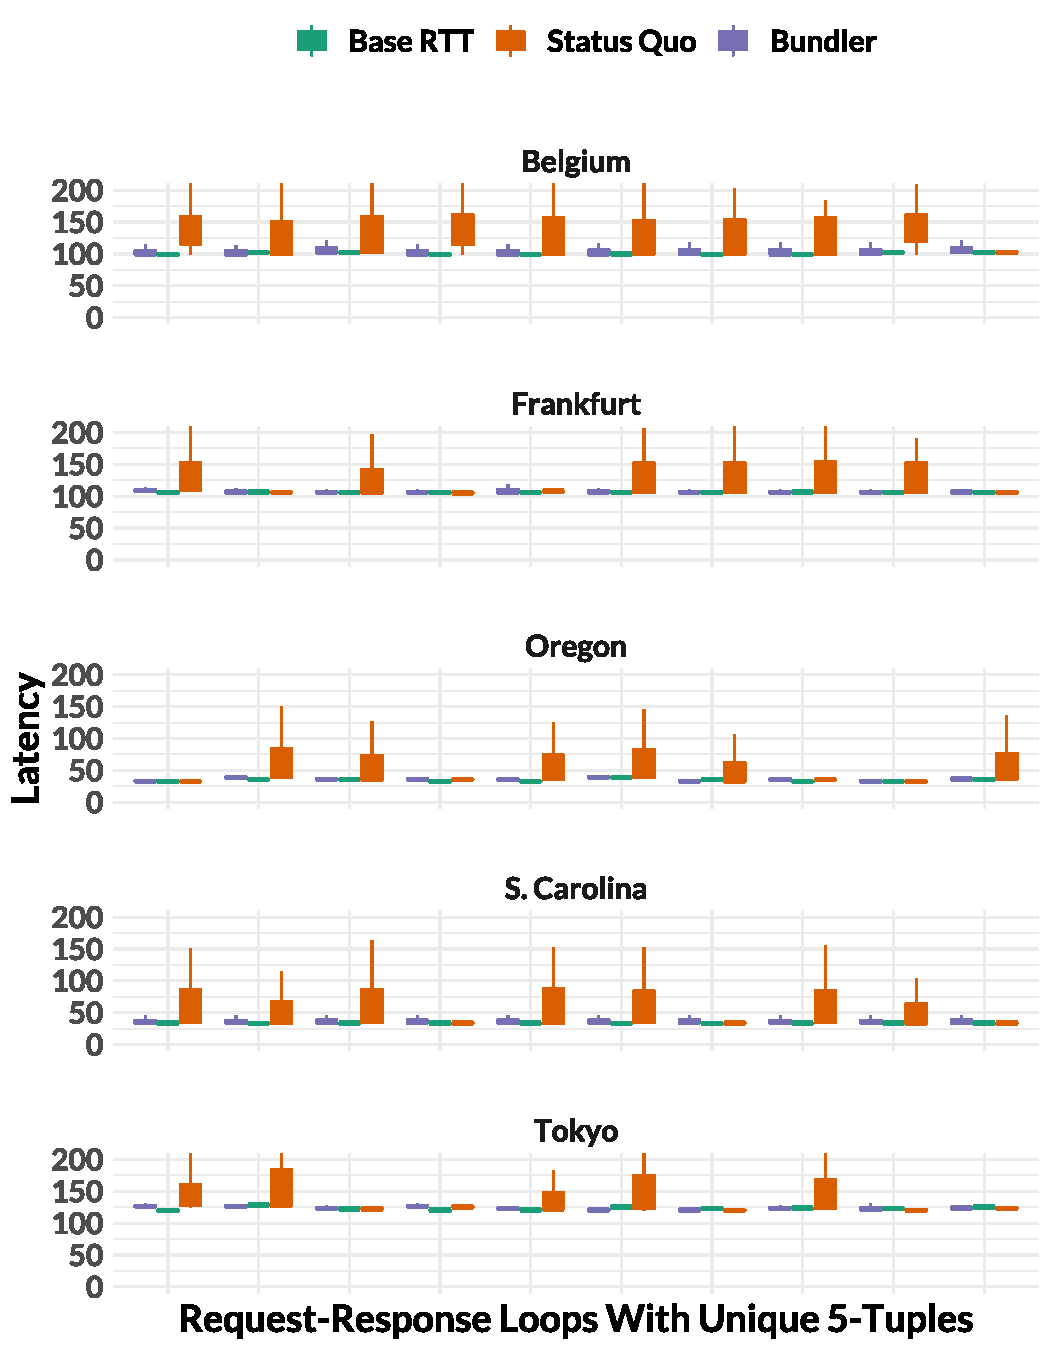
\includegraphics[width=\maxwidth]{figure/eval:realworld-1} 

\end{knitrout}
    \caption{On 5 real-Internet paths from the GCP datacenter in Iowa, \name achieves close to the Base RTT for latency-sensitive traffic. Each bar depicts an individual 5-tuple. On some paths, load-balancing in the Internet causes only some 5-tuples to experience queueing. \name offers scheduling for those paths.}
    \label{fig:eval:realworld}
\end{figure}
%\newcommand{\overviewBenefitsBundlerMedianImprovement}{round(100*(1-(overview_benefits_bundler_results[1] / overview_benefits_baseline_results[1])), 0)\%\xspace}

We next evaluate our prototype implementation on real Internet paths to answer three key questions that our emulated setup did not answer: (1) Does congestion (and queuing) actually occur in the middle of the network? (2) Is buffer-filling cross traffic rare enough in practice to ensure that \name provides a net improvement in performance? and (3) Is \name's design robust to multi-pathing effects in a real network?  
Our results reveal an affirmative answer for all three questions. We explain our experiment setup and results below. 

\Para{Experiment Setup} 
We deploy \name (\inbox) in a GCP datacenter in Iowa and generate traffic from multiple different machines in this datacenter (as detailed below). 
The generated traffic is sent to multiple machines in five different GCP datacenters (in Belgium, Frankfurt, Oregon, South Carolina, and Tokyo). We configured GCP to route traffic over the public Internet rather than a private network. 
We deploy a \name (\outbox) in each of these receiving datacenters, thus resulting in a total of five bundles spanning different regions of the globe.
We evaluate two different workloads in this setup: (i) Each bundle comprising of 10 parallel closed-loop 40 bytes UDP requests, where the sender issues a new request every time it receives a response. We measure the request-response RTTs in this workload to use as a baseline (and call them Base RTTs). (ii) We add 20 backlogged (\texttt{iperf}) flows to the above workload in each bundle. We run this workload both with and without \name and measure the UDP request-response RTTs (represented as \name and \baseline respectively). Effective SFQ across all flows with \name should not inflate the base request-response RTT.
We verified that the backlogged senders achieve similar throughput in all cases (2-4Gbit/s on these paths) both with and without \name, and that the \name machine in Iowa is not a bottleneck itself. 

\Para{Result} 
Figure~\ref{fig:eval:realworld} shows, for each of the five bundles, the resulting RTT box-plots for each of the ten request-response loops (with the 5 tuples in UDP/IP headers differing across all ten). 
We make the following key observations: (i) The \baseline RTTs are significantly higher than the Base RTT, which indicates significant in-network queueing. (ii) \name is able to move these queues and enforce SFQ scheduling effectively, resulting in request-response RTTs comparable to Base RTTs, and \realworldMedianLatencyImprovement smaller than \baseline at the median.
(iii) The \baseline results further reveal that different request-response loops within a given bundle see different amounts of queueing in the network. This indicates possible ECMP load-balancing in the network based on the 5 tuples, and how \name is robust to its effects.

